Lissajous figures are intricate patterns that appear on an oscilloscope when two periodic signals-often sinusoidal but also including square or triangular waves-are displayed simultaneously on the horizontal and vertical axes. Named after physicist Jules Antoine Lissajous, these figures visually represent the relationship between the frequencies and phase differences of the signals. The resulting pattern varies depending on the frequency ratio, phase shift, and waveform type. While sinusoidal waveforms typically produce smooth, predictable patterns, other waveforms like square or triangular waves can create more complex or sharper figures. Lissajous figures serve as valuable tools for analyzing signal relationships in various applications, including frequency measurement and phase analysis.

\subsection{Some Examples and their Mathematical proofs}
\begin{enumerate}
\item \textbf{\large \textbf{$x = A_0 si(\omega t)$} and \textbf{$y = A_0 sin(\omega t )$}},
\begin{figure}[h!]
    \centering
    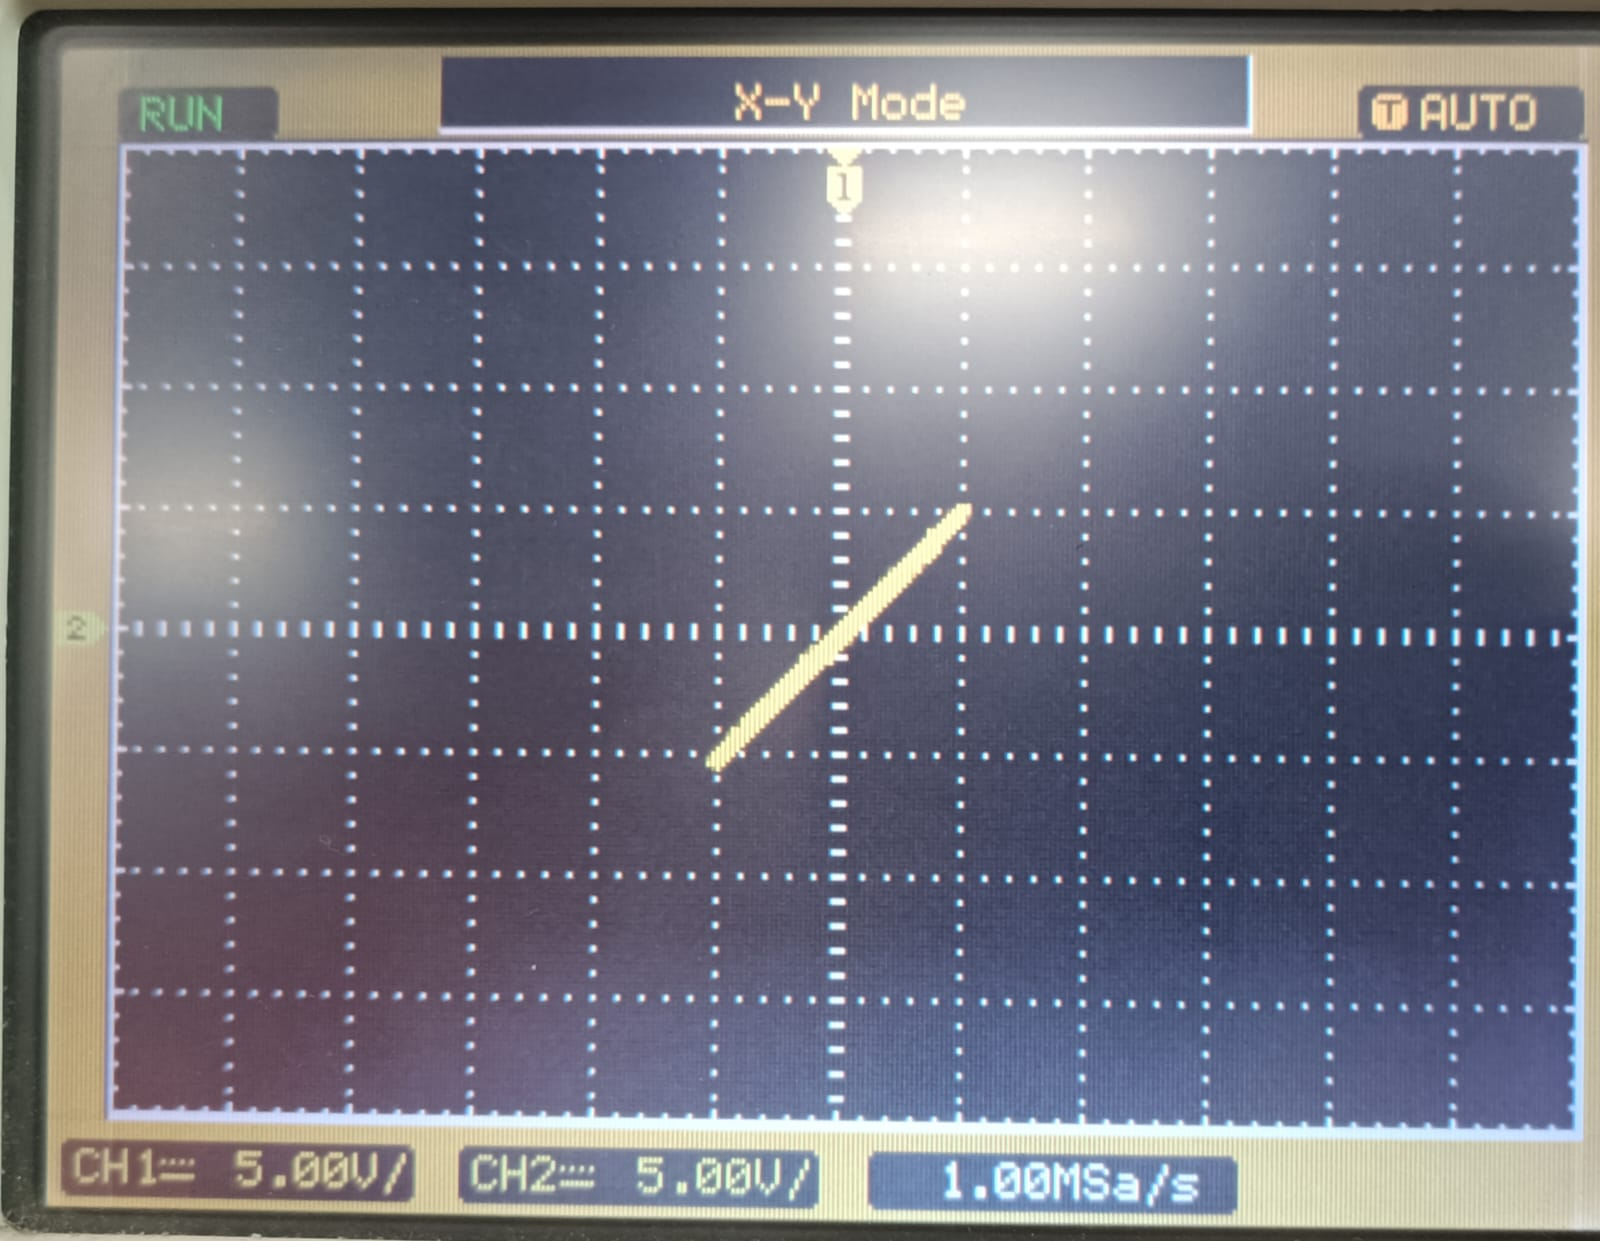
\includegraphics[width=0.6\textwidth]{actualgraph/line.jpeg}
    
    \caption{Graph of above signal using  Oscilloscope}
    \label{fig:sample_image}
    \end{figure}

    Mathematical proof,\\
    \[
    x=\sin(\omega t)
    \]
    \[
    y=\sin(\omega t )
    \]
    Now we can say , that \\
    $x=y$\\
    Therefore, it forms a straight line passing through origin and have slope 1.
    \begin{figure}[h!]
    \centering
    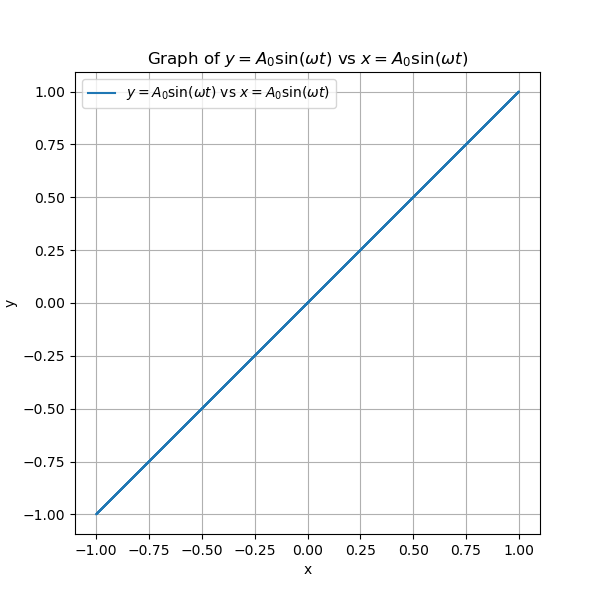
\includegraphics[width=0.6\textwidth]{graphs/Figure_2.png}
    \caption{Graph of above signal using python}
    \label{fig:sample_image}
     \end{figure}





\item   \textbf{\large \textbf{$x = A_0 sin(\omega t)$} and \textbf{$y = A_0 sin(\omega t + \frac{\pi}{2})$}},
    \begin{figure}[h!]
    \centering
    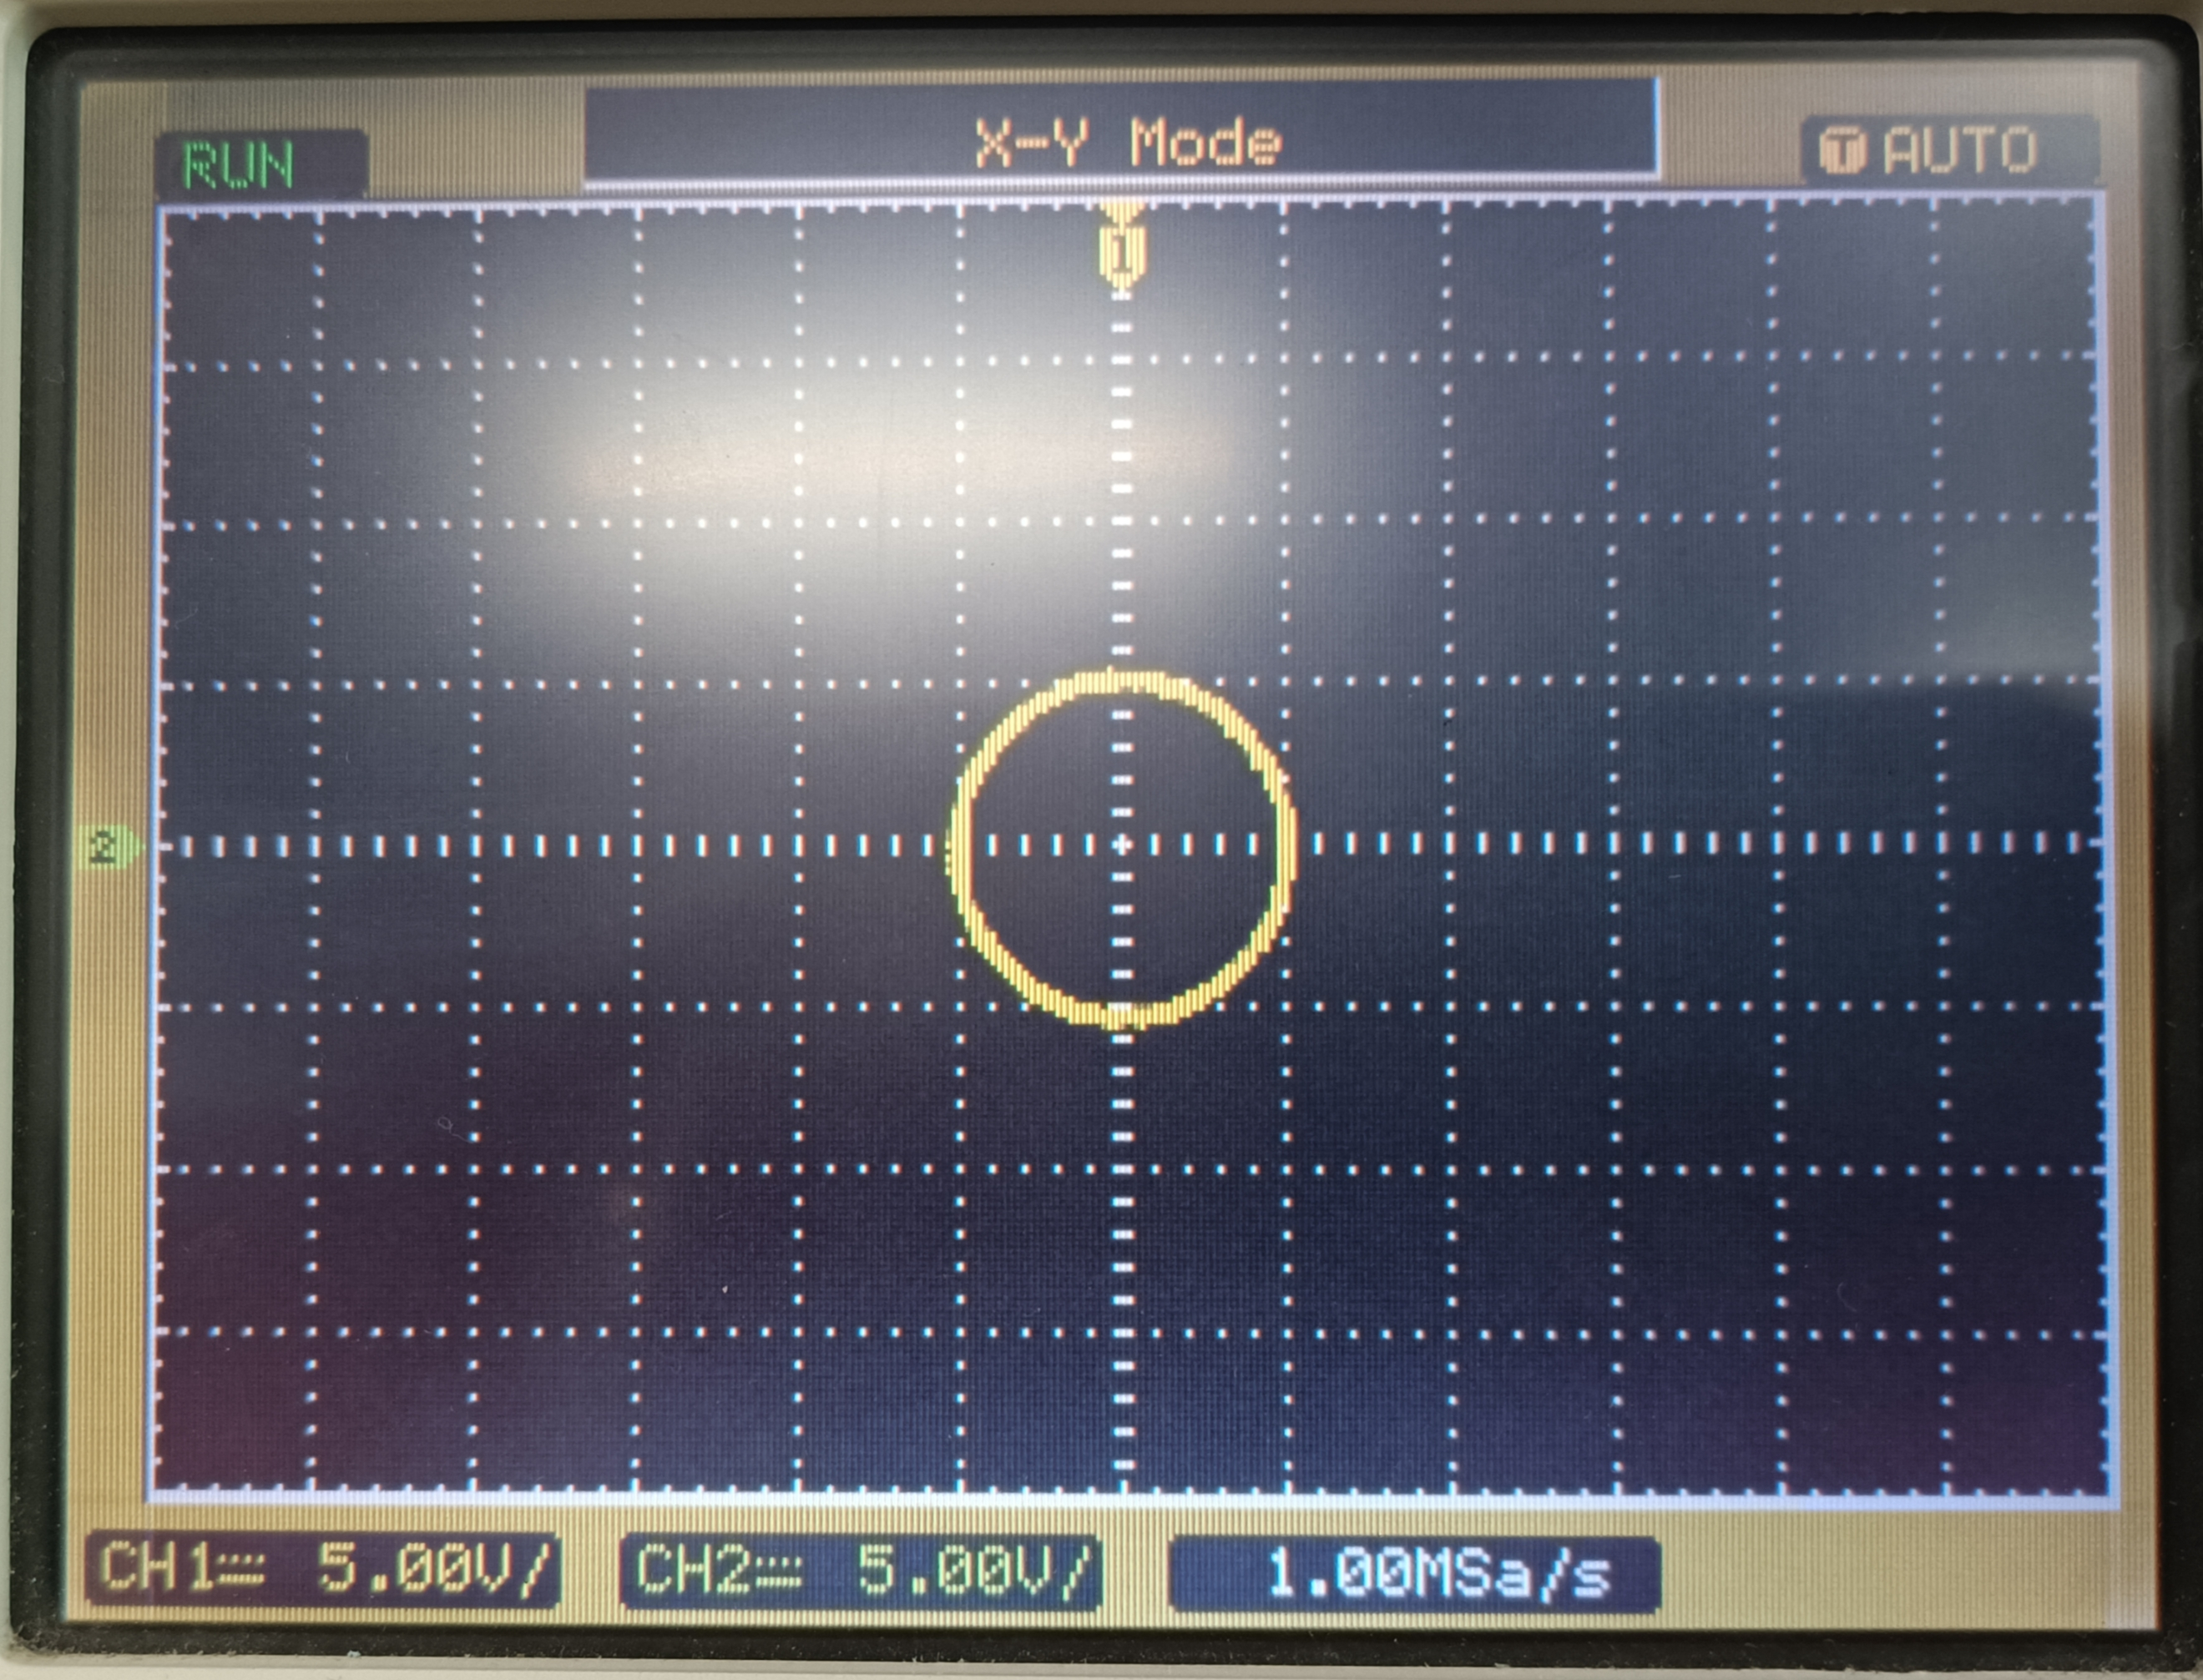
\includegraphics[width=0.6\textwidth]{actualgraph/circle.jpg}
    
    \caption{Graph of above signal using  Oscilloscope}
    \label{fig:sample_image}
    \end{figure}
(Here, Value of $\omega=2\pi 200$Hz)\\
Mathematical proof,\\
  \\ We consider two traveling waves with the same amplitude, frequency, and wavenumber but with a phase difference of \(90^\circ\):
\[
x(t) = A \sin(kx - \omega t) \quad \text{(wave along the \(x\)-axis)},
\]
\[
y(t) = A \sin\left(kx - \omega t + \frac{\pi}{2}\right) \quad \text{(wave along the \(y\)-axis)}.
\]
Using the trigonometric identity:
\[
\sin\left(kx - \omega t + \frac{\pi}{2}\right) = \cos(kx - \omega t),
\]
the equations become:
\[
x(t) = A \sin(kx - \omega t), \quad y(t) = A \cos(kx - \omega t).
\]
Resultant Curve,\\
To find the resultant curve, we eliminate \(t\) from the parametric equations. Using the Pythagorean identity:
\[
\sin^2\theta + \cos^2\theta = 1,
\]
we have:
\[
x^2 + y^2 = A^2 \sin^2(kx - \omega t) + A^2 \cos^2(kx - \omega t) = A^2.
\]
This is the equation of a \textbf{circle} with radius \(A\).

\begin{figure}[h!]
    \centering
    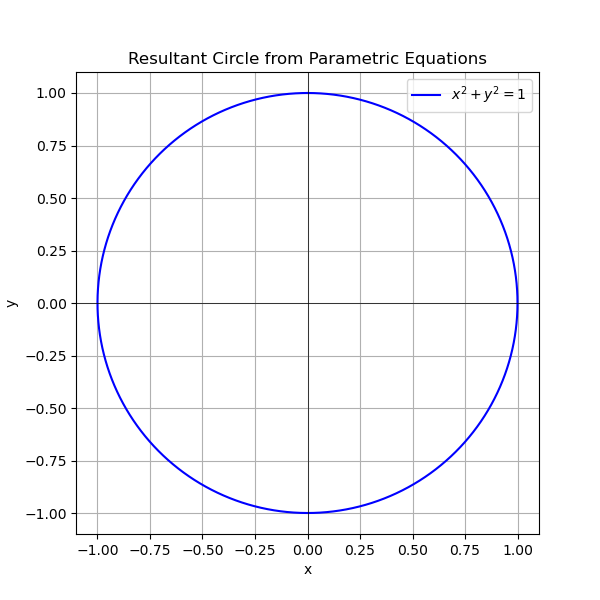
\includegraphics[width=0.3\textwidth]{graphs/1.png}
    \caption{Graph of above signal using python}
    \label{fig:sample_image}
     \end{figure}



\newpage
     
\item \textbf{\large \textbf{$x = A_0 sin(\omega t)$} and \textbf{$y = A_0 sin(\omega t + \frac{\pi}{4})$}},\\
     \begin{figure}[h!]
    \centering
    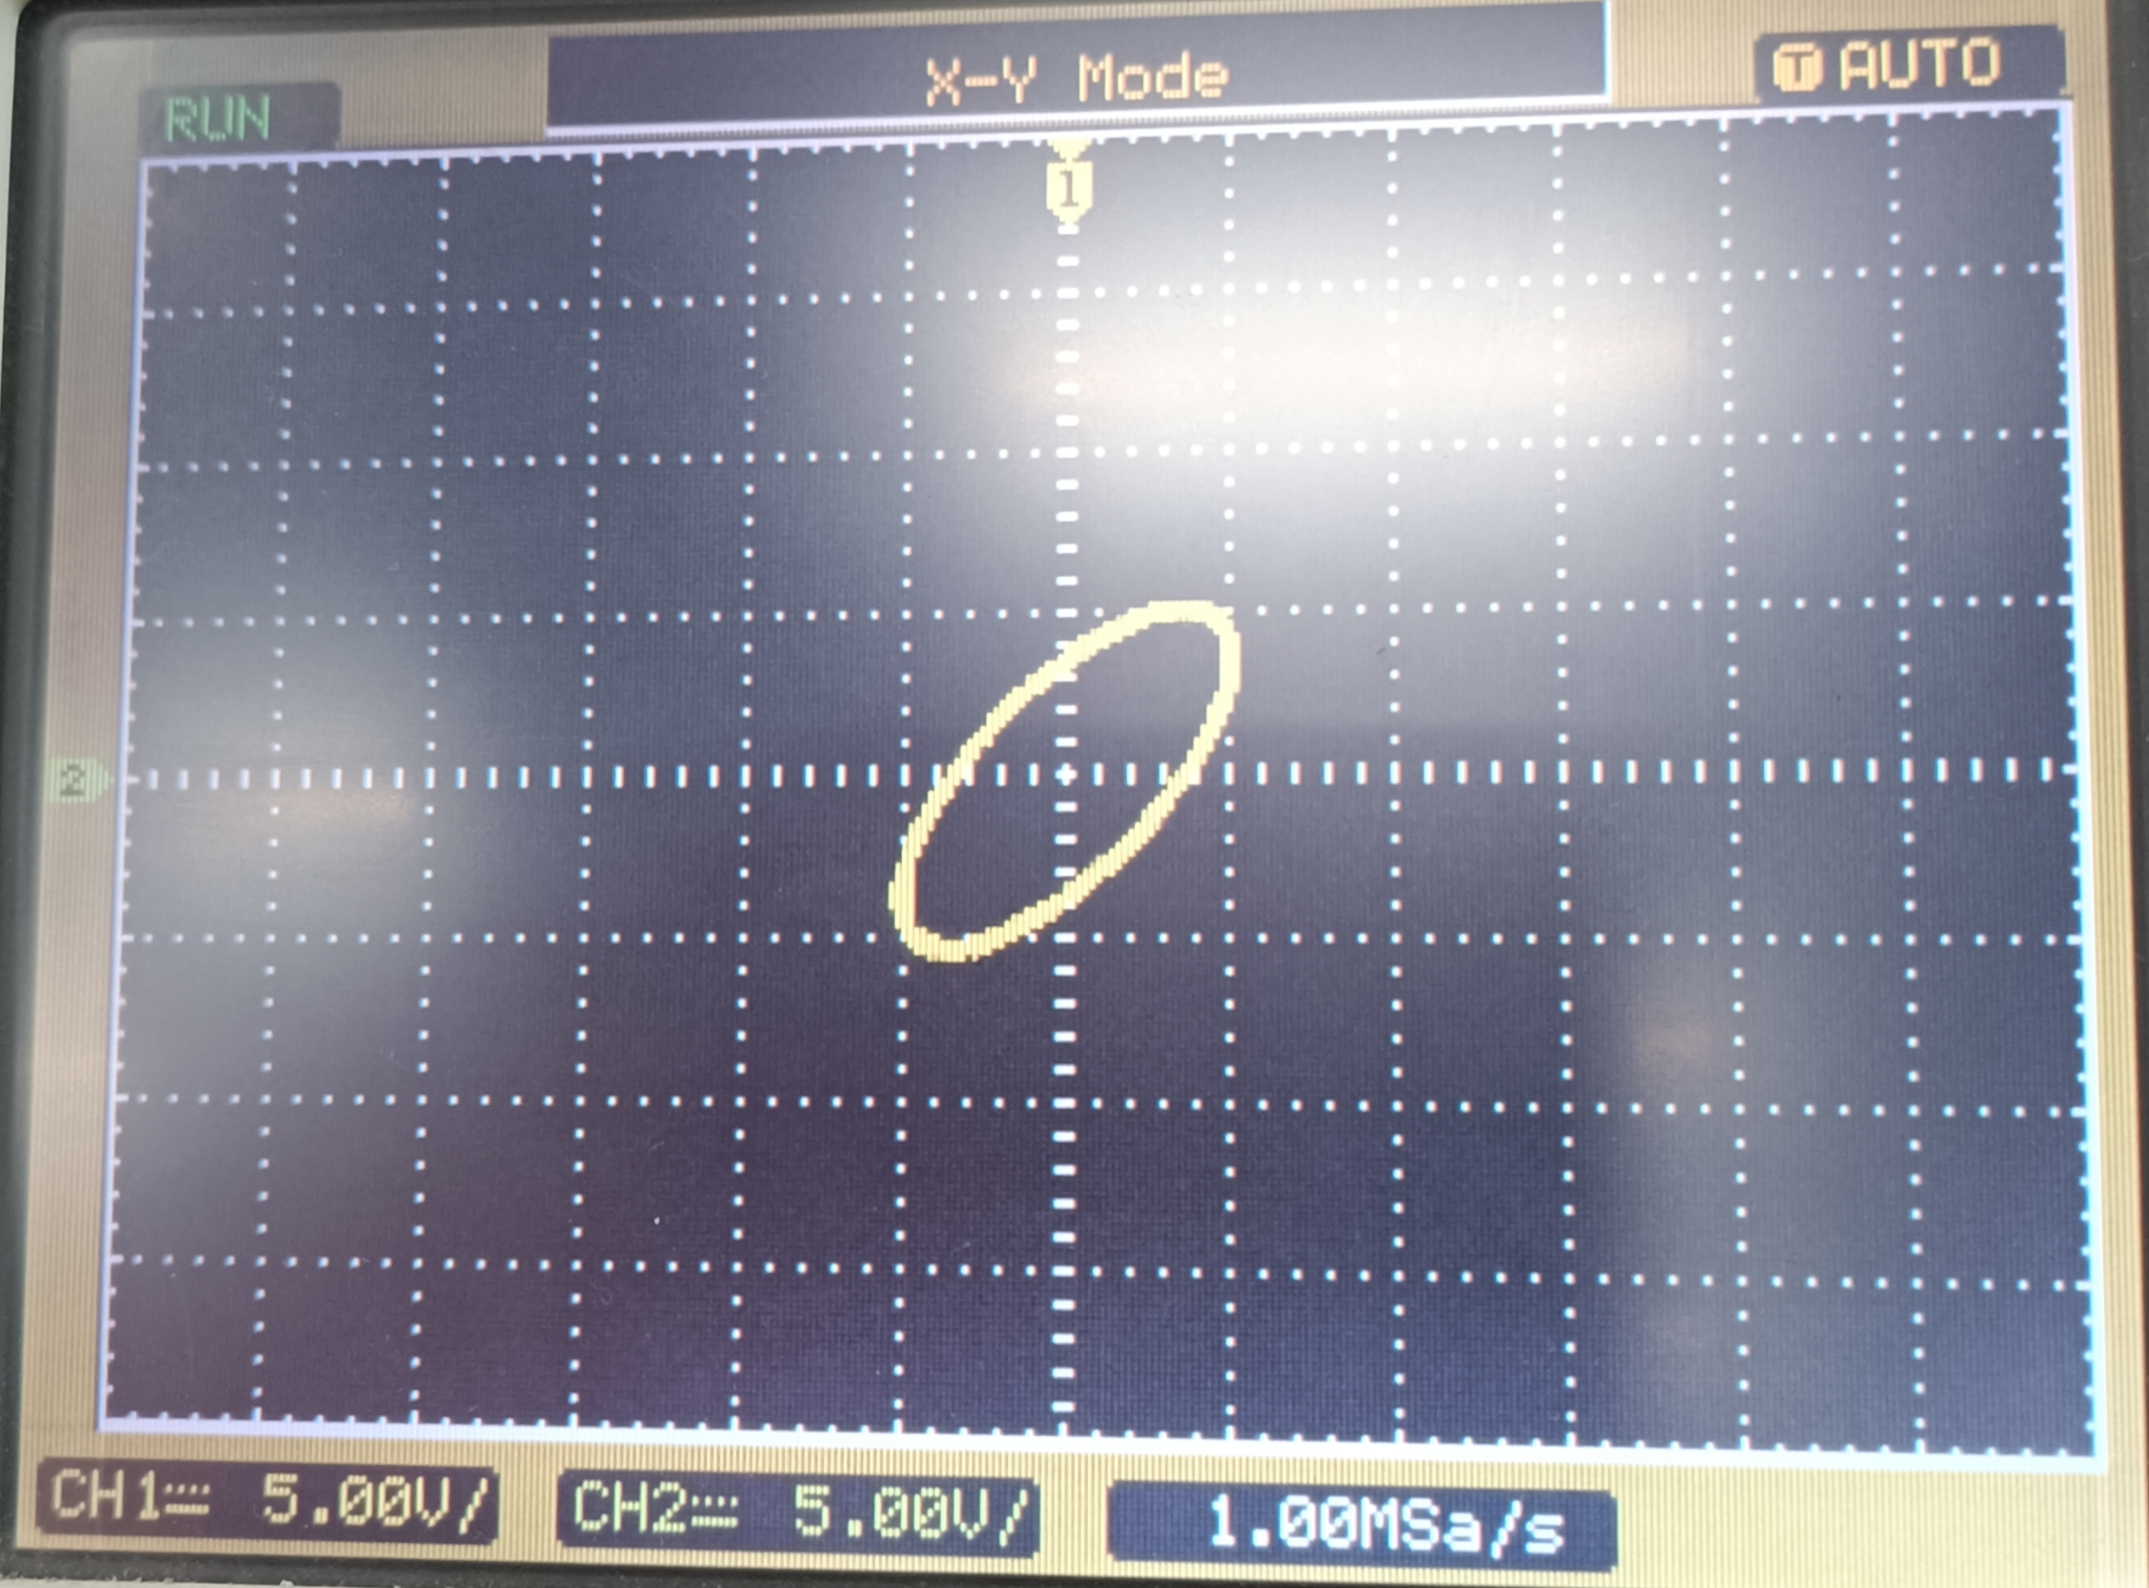
\includegraphics[width=0.6\textwidth]{actualgraph/ellipse.jpg}
    \caption{Graph of above signal using  Oscilloscope}
    \label{fig:sample_image}
    \end{figure}
Mathematical proof,\\
Express \( y \) in terms of \( x \),\\
We begin by rewriting the second equation for \( y \):
\[
y = A_0 \sin\left(\omega t + \frac{\pi}{4}\right)
\]
Using the trigonometric identity for \( \sin(A + B) \):
\[
\sin(A + B) = \sin A \cos B + \cos A \sin B,
\]
we get:
\[
y = A_0 \left[\sin(\omega t) \cos\left(\frac{\pi}{4}\right) + \cos(\omega t) \sin\left(\frac{\pi}{4}\right)\right]
\]
Since \( \cos\left(\frac{\pi}{4}\right) = \sin\left(\frac{\pi}{4}\right) = \frac{\sqrt{2}}{2} \), this simplifies to:
\[
y = A_0 \left[\frac{\sqrt{2}}{2} \sin(\omega t) + \frac{\sqrt{2}}{2} \cos(\omega t)\right]
\]
Now, using the first equation \( \sin(\omega t) = \frac{x}{A_0} \), we substitute into the above expression:
\[
y = \frac{A_0 \sqrt{2}}{2} \left( \frac{x}{A_0} + \cos(\omega t) \right)
\]
\[
y=\frac{1}{\sqrt{2}}x+\cos(\omega t)
\]
\[
y-\frac{1}{\sqrt{2}}x=\cos(\omega t)\frac{1}{\sqrt{2}}
\]
Squaring on Both sides,\\
\[
2y^2+x^2-2\sqrt{2}xy={A_0}^2-x^2
\]
\[
x^2+y^2+\sqrt{2}xy={A_0}^2
\]
Therefore, it is an ellipse.
  \begin{figure}[h!]
    \centering
    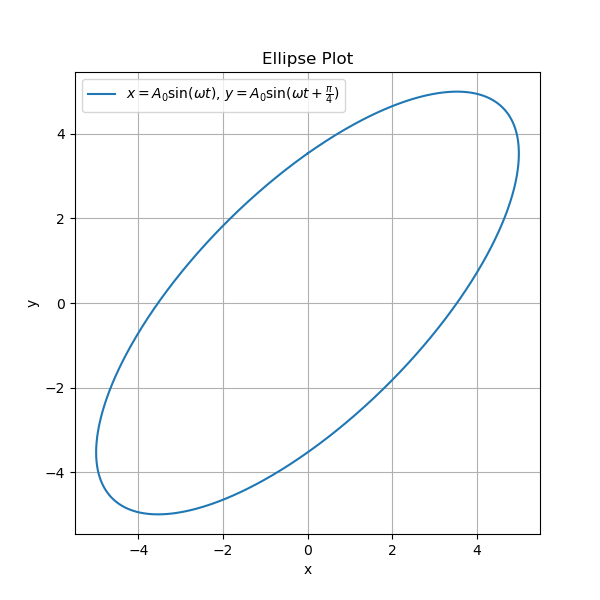
\includegraphics[width=0.4\textwidth]{graphs/Figure_1.png}
    \caption{Graph of above signal using python code}
    \label{fig:sample_image}
    \end{figure}








\newpage
\item \textbf{\large \textbf{$x = A_0 \sin(\omega t)$} and \textbf{$y = A_0 \sin(2\omega t)$}},
\begin{figure}[h!]
\centering
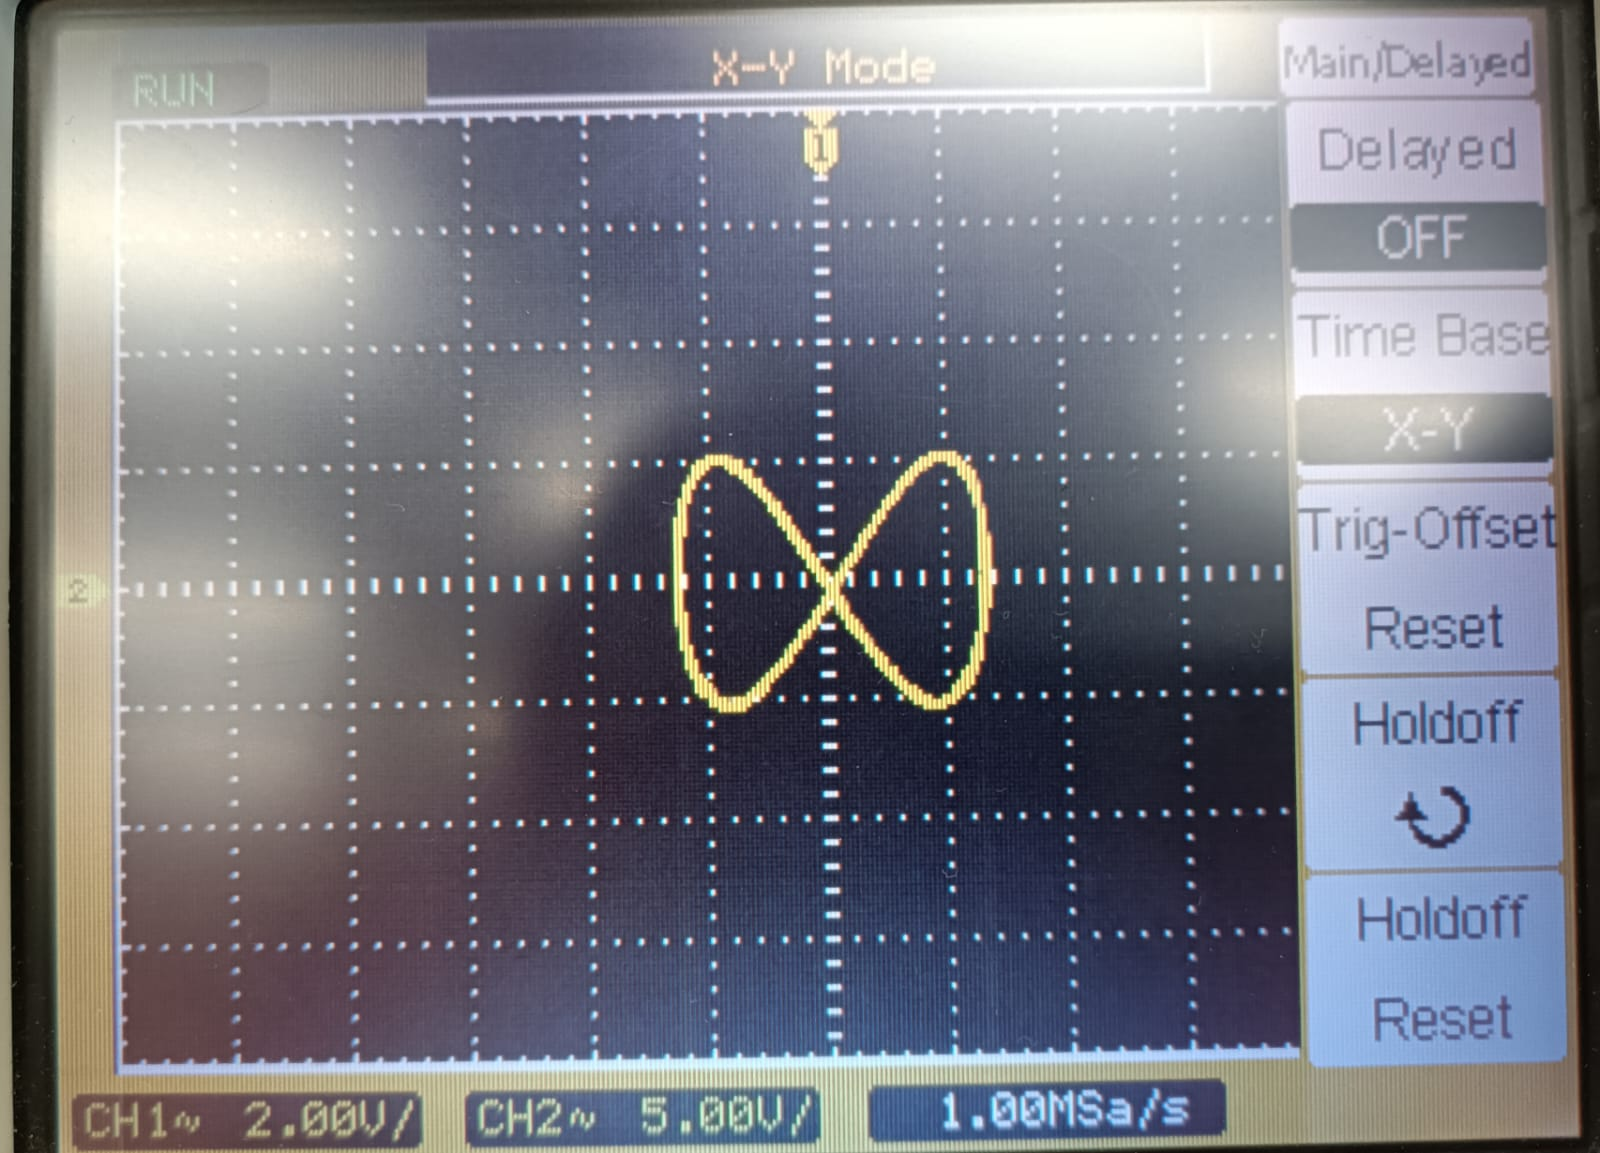
\includegraphics[width=0.6\textwidth]{actualgraph/infin.jpeg}
\caption{Graph of the above signal using Oscilloscope}
\label{fig:sample_image}
\end{figure}\\
Mathematical proof,\\
1. Using the trigonometric identity for \( \sin(2\theta) \):
\[
\sin(2\omega t) = 2 \sin(\omega t) \cos(\omega t),
\]
we substitute into \( y \):
\[
y = A_0 \cdot 2 \sin(\omega t) \cos(\omega t).
\]
\[
y = 2 A_0 \cos(\omega t) \cdot \sin(\omega t).
\]

2. From \( x = A_0 \sin(\omega t) \), solve for \( \sin(\omega t) \):
\[
\sin(\omega t) = \frac{x}{A_0}.
\]

3. Substitute \( \sin(\omega t) \) into the equation for \( y \):
\[
y = 2 A_0 \cos(\omega t) \cdot \frac{x}{A_0}.
\]
\[
y = 2 x \cos(\omega t).
\]

4. Use the Pythagorean identity \( \sin^2(\omega t) + \cos^2(\omega t) = 1 \) to solve for \( \cos(\omega t) \):
\[
\cos^2(\omega t) = 1 - \sin^2(\omega t).
\]
Substitute \( \sin(\omega t) = \frac{x}{A_0} \):
\[
\cos^2(\omega t) = 1 - \left(\frac{x}{A_0}\right)^2.
\]
\[
\cos(\omega t) = \pm\sqrt{1 - \frac{x^2}{A_0^2}}.
\]

5. Substitute \( \cos(\omega t) \) back into \( y \):
\[
y = 2 x \cdot \pm\sqrt{1 - \frac{x^2}{A_0^2}}.
\]


\begin{figure}[h!]
    \centering
    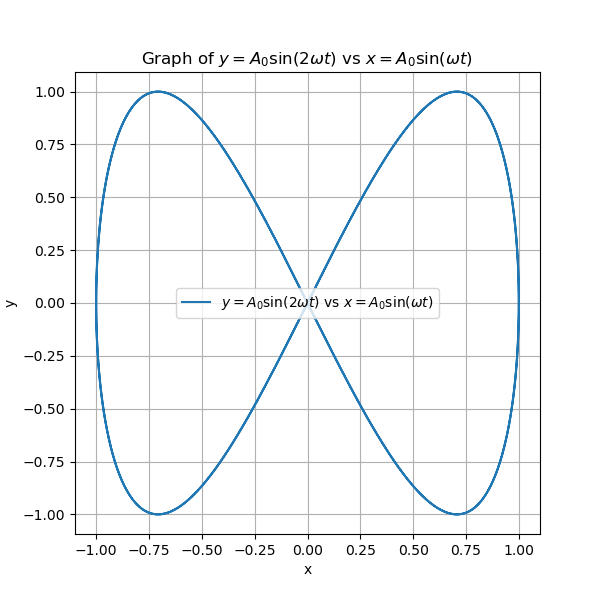
\includegraphics[width=0.3\textwidth]{graphs/Figure_3.png}
    \caption{Graph of the above signal using Python code}
    \label{fig:sample_image}
\end{figure}







\newpage
\item \textbf{\large \textbf{$x = A_0 \sin(\omega t)$} and \textbf{$y = A_0 \sin(3\omega t)$}}\\
 \begin{figure}[h!]
    \centering
    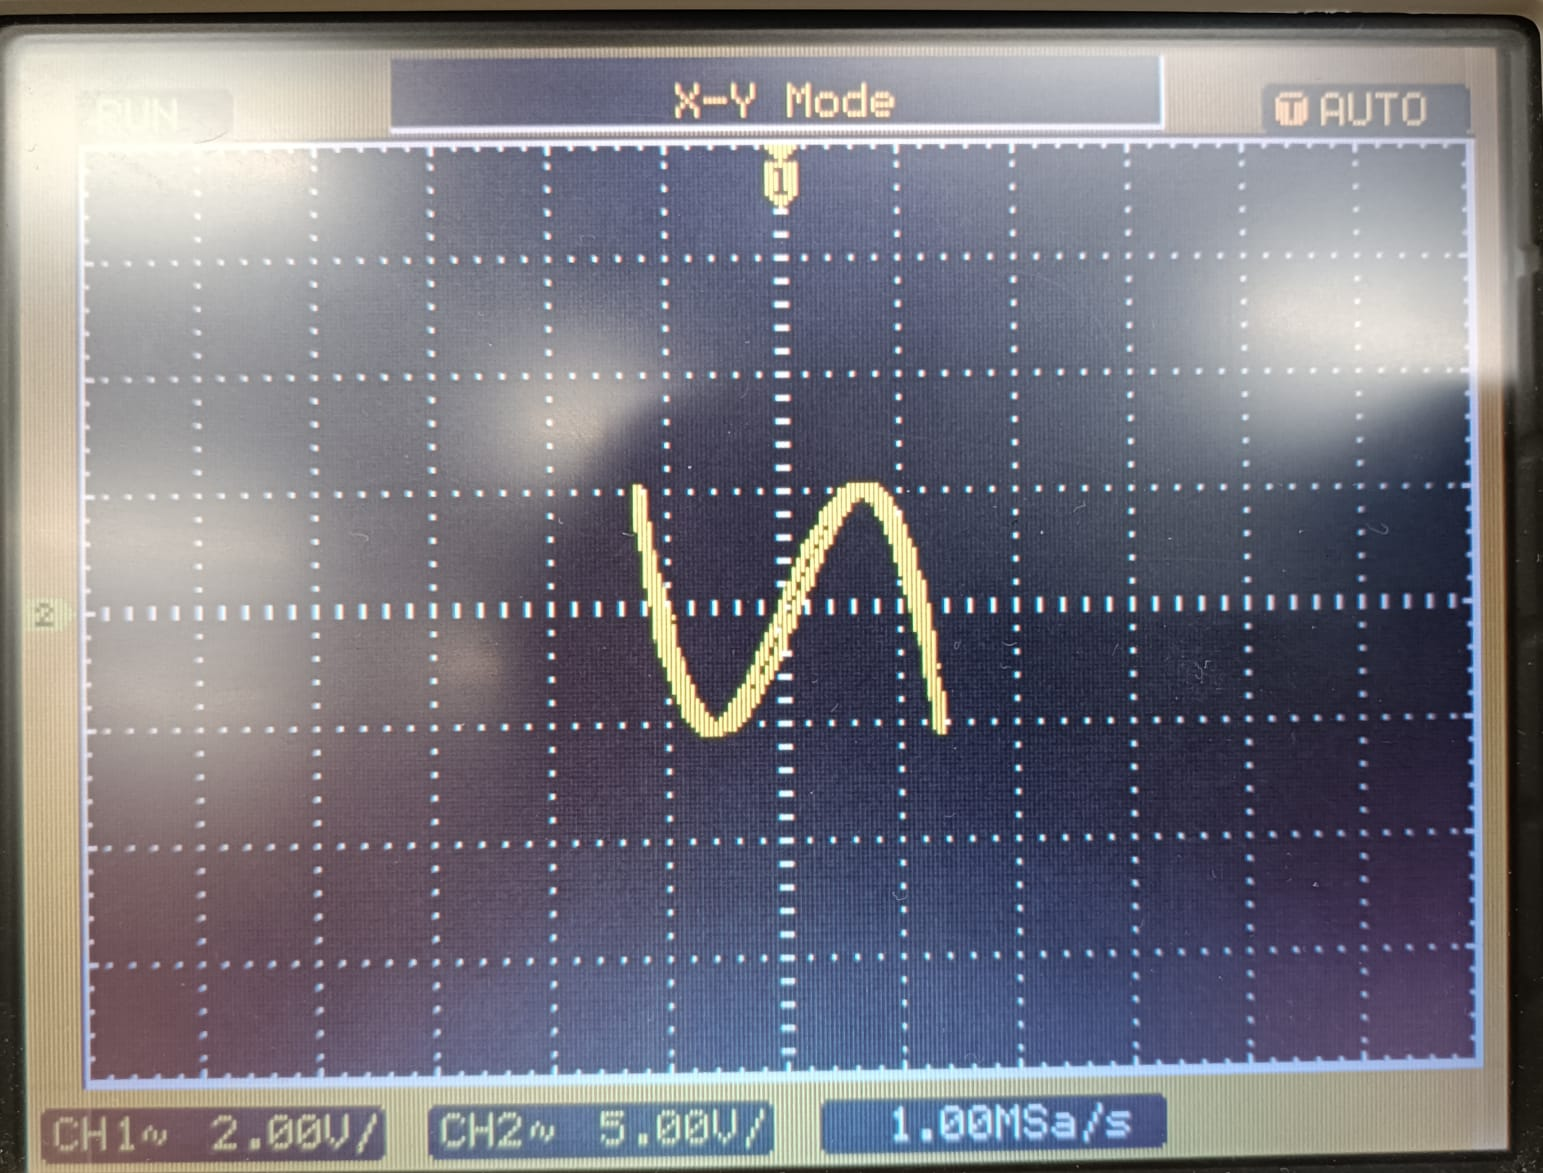
\includegraphics[width=0.3\textwidth]{actualgraph/3sin.jpeg}
    \caption{Graph of above signal in oscilloscope}
    \label{fig:sample_image}
    \end{figure}
Using the trigonometric identity for \(\sin(3\theta)\):
\[
\sin(3\omega t) = 3\sin(\omega t) - 4\sin^3(\omega t),
\]

we substitute \(\sin(\omega t) = \frac{x}{A_0}\) (from \(x = A_0 \sin(\omega t)\)) into \(y = A_0 \sin(3\omega t)\):
\[
y = A_0 \left[3\sin(\omega t) - 4\sin^3(\omega t)\right]
\]
\[
y = A_0 \left[3\frac{x}{A_0} - 4\left(\frac{x}{A_0}\right)^3\right]
\]

Simplify:
\[
y = 3x - \frac{4x^3}{A_0^2}.
\]

The final relationship is:
\[
y = 3x - \frac{4x^3}{A_0^2}.
\]
 \begin{figure}[h!]
    \centering
    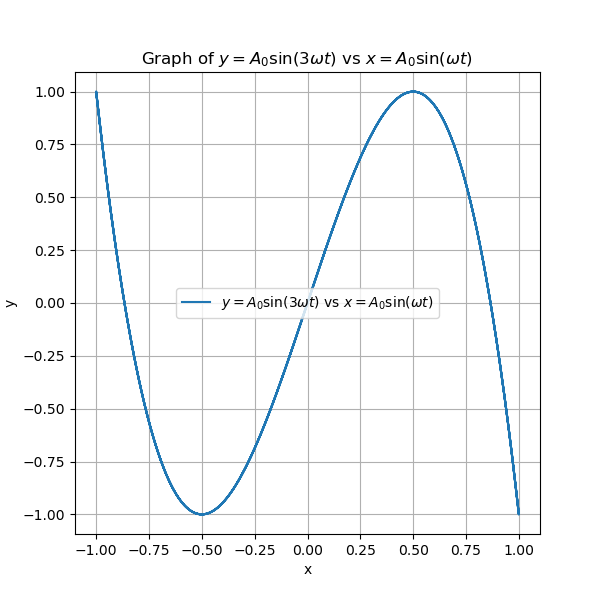
\includegraphics[width=0.3\textwidth]{graphs/Figure_4.png}
    \caption{Graph of above signal using python}
    \label{fig:sample_image}
     \end{figure}

\item \textbf{\large \textbf{$x = A_0 \sin(\omega t)$} and \textbf{$y = A_0 \sin(2\omega t+\frac{\pi}{2})$}},\\
\begin{figure}[h!]
    \centering
    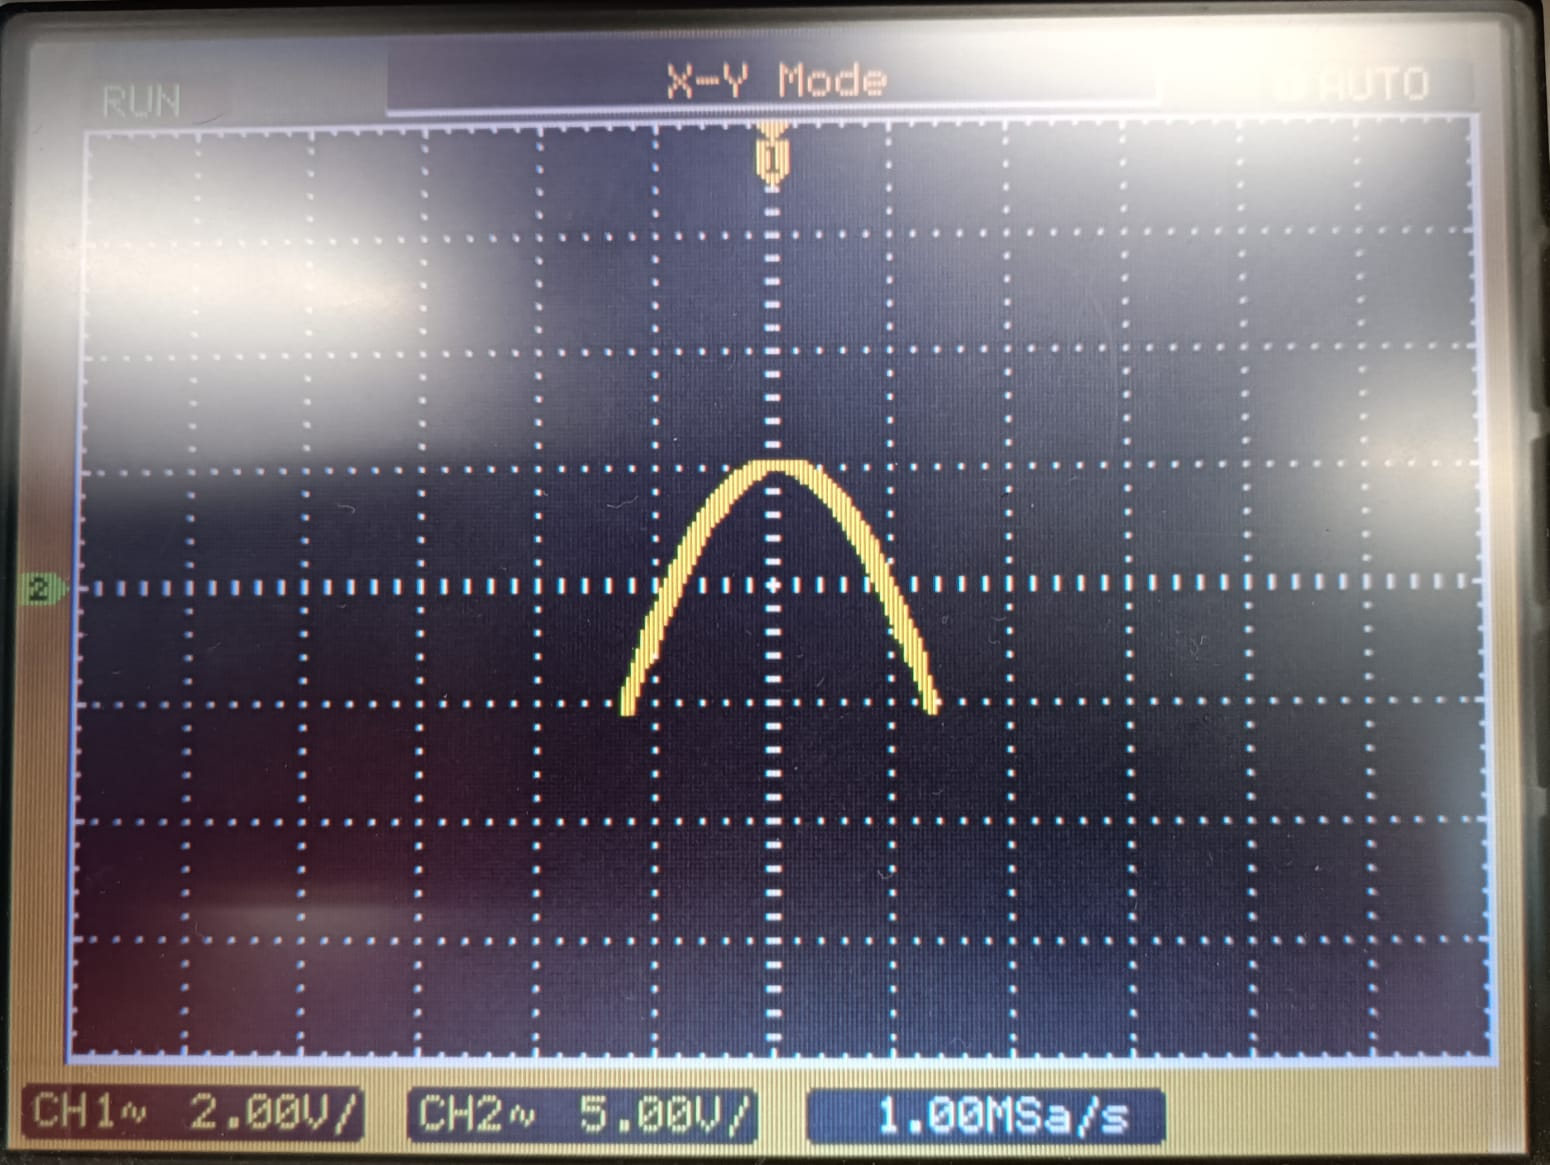
\includegraphics[width=0.6\textwidth]{actualgraph/parab.jpeg}
    \caption{Graph of above signal in oscilloscope}
    \label{fig:sample_image}
     \end{figure}

Mathematical proof,\\
\[
x = A_0 \sin(\omega t)\\
\]
\[
y = A_0 \sin(2\omega t+\frac{\pi}{2})\\
\]
\[
y= A_0 \cos(2\omega t)
\]
\[
y=A_0(1-2\sin^2(\omega t))
\]
\[
\implies y= A_0(1-2(\frac{x}{A_0})^2)
\]
Therefore, it is a parabola passing through y axis $A_0$
\begin{figure}[h!]
    \centering
    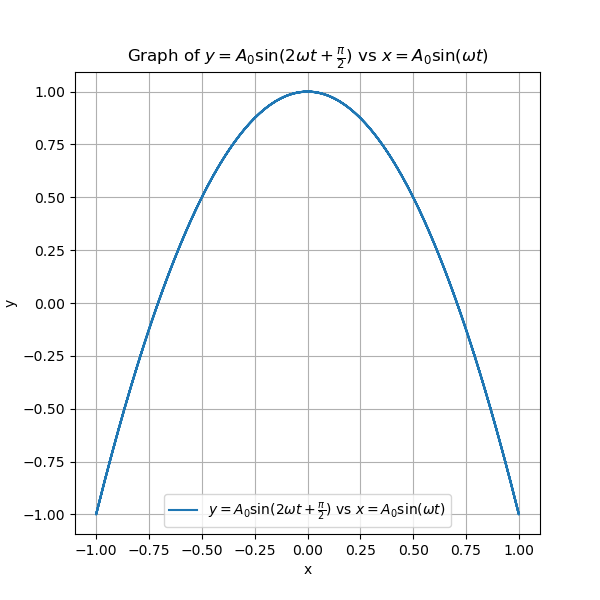
\includegraphics[width=0.4\textwidth]{graphs/Figure_5.png}
    \caption{Graph of above signal using python}
    \label{fig:sample_image}
     \end{figure}

\end{enumerate}